% =====================================================================
%  Beneath the Mesa -- ENG 220 Project Report (Team 23)
%  Two-column report template styled to match the project proposal:
%  Palatino (URW Palladio) text, navy headings, blue rules and header.
%
%  Build:  pdflatex report -> bibtex report -> pdflatex report (x2)
%          (or `latexmk -pdf report.tex`; Overleaf does this automatically)
%
%  Orange [notes] mark what still needs to be written.
%  Dashed boxes mark figures that still need to be made.
% =====================================================================
\documentclass[10pt,twocolumn,letterpaper]{article}

% ---------------------------------------------------------------------
%  Switches
% ---------------------------------------------------------------------
\newif\ifdraftnotes \draftnotestrue   % \draftnotesfalse hides every [orange note]
\newif\ifcoverpage  \coverpagefalse   % \coverpagetrue adds a proposal-style cover page
\newif\ifroughdraft \roughdrafttrue    % \roughdraftfalse removes the red ROUGH DRAFT stamp

% ---------------------------------------------------------------------
%  Fonts and text
% ---------------------------------------------------------------------
\usepackage[T1]{fontenc}
\usepackage[utf8]{inputenc}
\usepackage{mathpazo}                 % URW Palladio, the proposal's typeface
\usepackage[protrusion=true,expansion=true]{microtype}
\usepackage{amsmath}

% ---------------------------------------------------------------------
%  Page layout
% ---------------------------------------------------------------------
\usepackage[letterpaper,top=0.8in,bottom=0.85in,left=0.75in,right=0.75in,
            columnsep=0.28in,headheight=20pt,headsep=8pt,footskip=26pt]{geometry}
\setlength{\parindent}{1.2em}
\setlength{\parskip}{0pt}

% ---------------------------------------------------------------------
%  Colors (sampled from the proposal PDF)
% ---------------------------------------------------------------------
\usepackage{xcolor}
\definecolor{titleblue}{RGB}{23,54,93}     % #17365D  headings, title
\definecolor{accentblue}{RGB}{54,95,145}   % #365F91  rules, header, links
\definecolor{tintblue}{RGB}{237,241,247}   % light panel fill
\definecolor{draftorange}{RGB}{190,84,20}  % draft notes only
\definecolor{draftred}{RGB}{192,0,0}       % ROUGH DRAFT stamp

% ---------------------------------------------------------------------
%  Headings
% ---------------------------------------------------------------------
\usepackage{titlesec}
\usepackage{needspace}
\usepackage{etoolbox}
\titleformat{\section}{\color{titleblue}\large\bfseries}{\thesection}{0.55em}{}
  [{\color{accentblue}\titlerule[0.6pt]}]
\titlespacing*{\section}{0pt}{2.0ex plus 0.6ex minus 0.3ex}{1.0ex}
\titleformat{\subsection}{\color{accentblue}\normalsize\bfseries}{\thesubsection}{0.55em}{}
\titlespacing*{\subsection}{0pt}{1.4ex plus 0.4ex minus 0.2ex}{0.5ex}
\titleformat{\subsubsection}[runin]{\normalsize\bfseries\itshape}{}{0pt}{}[.]
\titlespacing*{\subsubsection}{0pt}{1.0ex plus 0.3ex}{0.6em}
\pretocmd{\section}{\Needspace{4\baselineskip}}{}{}       % keep headings with their text
\pretocmd{\subsection}{\Needspace{3\baselineskip}}{}{}

% ---------------------------------------------------------------------
%  Running header and footer (same as the proposal)
% ---------------------------------------------------------------------
\usepackage{fancyhdr}
\pagestyle{fancy}
\fancyhf{}
\fancyhead[L]{\small\color{accentblue}Project Report}
\fancyhead[R]{\small\color{accentblue}Aquifer \& Well Resources: Sandoval County, NM}
\fancyfoot[C]{\small\thepage}
\renewcommand{\headrulewidth}{0.4pt}
\renewcommand{\headrule}{\hbox to\headwidth{\color{accentblue}\leaders\hrule height\headrulewidth\hfill}}

\fancypagestyle{firstpage}{%
  \fancyhf{}%
  \renewcommand{\headrulewidth}{0pt}%
  \fancyfoot[L]{\footnotesize\color{accentblue}ENG 220 Project Report \,\textbullet\, Team 23 \,\textbullet\, \reportstatus}%
  \fancyfoot[R]{\small\thepage}%
}

% ---------------------------------------------------------------------
%  Lists, tables, figures, captions
% ---------------------------------------------------------------------
\usepackage{enumitem}
\setlist{itemsep=1pt,topsep=3pt,parsep=0pt}
\setlist[itemize]{leftmargin=1.2em,label={\color{accentblue}\textbullet}}
\usepackage{booktabs,tabularx,array}
\renewcommand{\arraystretch}{1.12}
\usepackage{graphicx}
\graphicspath{{figures/}}
\usepackage{caption}
\captionsetup{font=small,labelfont={bf,color=titleblue},labelsep=period,justification=justified}
\captionsetup[table]{position=top,skip=4pt}  % for tables you add later
\usepackage{tikz}
\usepackage{stfloats}                 % lets full-width figures sit at the page bottom too

% ---------------------------------------------------------------------
%  References and links
% ---------------------------------------------------------------------
\usepackage[round,authoryear]{natbib}
\setlength{\bibsep}{2.5pt}
\renewcommand{\bibfont}{\small\raggedright}
\usepackage{xurl}
\usepackage[colorlinks=true,linkcolor=accentblue,citecolor=accentblue,urlcolor=accentblue,
            pdftitle={Beneath the Mesa: Aquifer and Well Water Resources Across Sandoval County, New Mexico},
            pdfauthor={Djordjevic, Gonzales, Wauneka, Watkins, Yousef}]{hyperref}
\urlstyle{same}

% ---------------------------------------------------------------------
%  Draft helpers
% ---------------------------------------------------------------------
\newcommand{\reportstatus}{\ifroughdraft Rough draft, November 2, 2026\else Final, November 16, 2026\fi}
% Red stamp shown on page 1 and the cover page while \roughdrafttrue
\newcommand{\draftstamp}[1][\large]{\ifroughdraft%
  \tikz\node[draw=draftred,line width=1.1pt,rounded corners=2pt,inner xsep=9pt,inner ysep=4pt,
    text=draftred,font=#1\bfseries]{\textls[180]{ROUGH DRAFT}};\fi}
\newcommand{\draftnote}[1]{\ifdraftnotes{\color{draftorange}\itshape[#1]}\fi}
% Dashed box that stands in for a figure that does not exist yet.
%   \figplaceholder[height]{what the figure will show}
% When the figure is ready, save it in figures/ and replace the
% placeholder with:  \includegraphics[width=\linewidth]{file-name}
\newcommand{\figplaceholder}[2][1.8in]{%
  \begin{tikzpicture}
    \draw[accentblue!70,dashed,line width=0.6pt,fill=tintblue,rounded corners=2pt]
      (0,0) rectangle (\linewidth,#1);
    \node[text width=0.82\linewidth,align=center,font=\small\itshape,text=accentblue]
      at (0.5\linewidth,0.5*#1) {#2};
  \end{tikzpicture}}
\newcommand{\infohead}[1]{{\color{titleblue}\footnotesize\bfseries\MakeUppercase{#1}}\par\vspace{2pt}}

% =====================================================================
\begin{document}

% ---------------------------------------------------------------------
%  Optional cover page (same layout as the proposal cover)
% ---------------------------------------------------------------------
\ifcoverpage
\begin{titlepage}
  \centering
  \vspace*{1.6in}
  {\color{accentblue}\rule{\textwidth}{0.8pt}}\par\vspace{1.4em}
  {\color{titleblue}\fontsize{24}{29}\selectfont\bfseries Beneath the Mesa\par}
  \vspace{0.9em}
  {\color{accentblue}\fontsize{17}{22}\selectfont Assessing Aquifer and Well Water Resources\\
    Across Sandoval County, New Mexico\par}
  \vspace{1.3em}
  {\color{accentblue}\rule{\textwidth}{0.8pt}}\par\vspace{1.6em}
  {\itshape A County-Scale Screening Study with Cuba, New Mexico as a Focus Area\par}
  \vspace{1.3in}
  {\color{titleblue}\large\bfseries Project Report\par}
  \ifroughdraft\vspace{1.2em}\draftstamp[\Large]\par\vspace{-0.4in}\fi
  \vspace{1.2in}
  \begin{tabular}{@{}r@{\hspace{0.8em}}l@{}}
    \textbf{Course:}     & ENG 220 \\
    \textbf{Instructor:} & Ramiro Jordan \\
    \textbf{Team:}       & \#23 Petar Djordjevic, Dylan Gonzales, James Wauneka,\\
                         & \phantom{\#23 }Micah Watkins, Meckrem Yousef \\
    \textbf{Date:}       & \ifroughdraft November 2, 2026 (rough draft)\else November 16, 2026\fi \\
  \end{tabular}
  \vfill
\end{titlepage}
\fi

% ---------------------------------------------------------------------
%  Title block and abstract (full width)
% ---------------------------------------------------------------------
\twocolumn[{%
\begin{center}
  \ifroughdraft\vspace*{-1.5ex}\draftstamp\par\vspace{1.4ex}\fi
  {\color{accentblue}\rule{\textwidth}{0.8pt}}\par\vspace{0.9ex}
  {\color{titleblue}\fontsize{22}{26}\selectfont\bfseries Beneath the Mesa\par}
  \vspace{0.7ex}
  {\color{accentblue}\fontsize{14.5}{18}\selectfont Assessing Aquifer and Well Water Resources\\
    Across Sandoval County, New Mexico\par}
  \vspace{0.9ex}
  {\color{accentblue}\rule{\textwidth}{0.8pt}}\par\vspace{0.9ex}
  {\itshape A County-Scale Screening Study with Cuba, New Mexico as a Focus Area\par}
  \vspace{2.0ex}
  {\large Petar Djordjevic, Dylan Gonzales, James Wauneka, Micah Watkins, and Meckrem Yousef\par}
  \vspace{0.6ex}
  {\small ENG 220, Team 23 \,\textbullet\, Instructor: Ramiro Jordan\par}
\end{center}
\vspace{1.2ex}
{\color{accentblue}\rule{\textwidth}{0.4pt}}\par\vspace{1.4ex}
\noindent
\begin{minipage}[t]{0.25\textwidth}
  \raggedright\footnotesize
  \infohead{Report info}
  \ifroughdraft Status: {\color{draftred}\bfseries Rough draft}\\
  Date: November 2, 2026\\
  \else Status: Final\\
  \fi Final due: November 16, 2026\par\vspace{1.4ex}
  \infohead{Keywords}
  Groundwater\\ Aquifers\\ Wells\\ Sandoval County\\ Cuba, New Mexico\par\vspace{1.4ex}
  \infohead{Online}
  \href{https://eng220aquiferproject.streamlit.app/}{Interactive dashboard}\\
  \href{https://github.com/pdjordj11/eng_220_aquifer_project}{Code and data (GitHub)}\\
  \href{https://pdjordj11.github.io/eng_220_aquifer_project/}{Project documentation}
\end{minipage}%
\hfill{\color{accentblue}\vrule width 0.4pt}\hfill
\begin{minipage}[t]{0.70\textwidth}
  \infohead{Abstract}
  \small
  Water scarcity is a persistent challenge across New Mexico. Sandoval County spans several
  hydrogeologic settings, and its communities depend on a mix of groundwater wells, surface water,
  and acequia irrigation systems. This project focuses on groundwater: it evaluates the condition
  of the county's aquifers and wells, with Cuba, New Mexico, on the eastern edge of the San Juan
  Basin, as a focused case study. The project is motivated by concern about declining groundwater
  near Cuba, but rather than assume how severe that decline is or what is causing it, we test what
  the available public data actually show, and where they are too sparse to say. We combined
  public water-level, well, aquifer-test, geologic, and streamflow records from the USGS, the New
  Mexico Bureau of Geology, and the State Engineer, and analyzed them with reproducible code. Five
  of the nine long-term monitoring wells, all 65--95\,km from Cuba, fell over their 1998--2026
  records, while the Sandia site north of Albuquerque has risen about 13\,ft since 2007. Near Cuba,
  the only well records are one-time aquifer tests from 1957--1979, and no well within 25\,km has
  been measured repeatedly, so the data can neither confirm nor rule out severe depletion of Cuba's
  aquifer. Answering that question requires the village's own well records.
\end{minipage}
\par\vspace{1.6ex}
{\color{accentblue}\rule{\textwidth}{0.4pt}}\par\vspace{2.6ex}
}]
\thispagestyle{firstpage}

% =====================================================================
\section{Introduction}
% =====================================================================
\subsection{Background and Motivation}
\draftnote{Background on water resources in New Mexico and Sandoval County, and the concern about
declining groundwater near Cuba that motivated the project.}

\subsection{Approach}
The study works at two levels:
\begin{itemize}
  \item \textbf{County-wide screening.} Map and compare aquifers, wells, and groundwater levels
        across Sandoval County. Because the county crosses several geologic regions, comparisons
        are grouped by area and, where the records name it, by aquifer unit, instead of treating
        the county as one uniform aquifer.
  \item \textbf{Cuba case study.} A closer look at the Ojo Alamo Sandstone and San Jose Formation
        near Cuba, using published maps of both formations, aquifer-test records from nearby
        wells, and stream measurements on the Rio Puerco at Cuba.
\end{itemize}

\subsection{Research Questions}
\begin{enumerate}[label={\color{titleblue}\bfseries RQ\arabic*.},leftmargin=2.6em,labelsep=0.4em]
  \item How have groundwater levels changed at monitored wells in Sandoval County, and which wells
        show sustained decline, stability, or recovery?
  \item What do well records show about well depth, depth to water, and the aquifer units that
        wells in different parts of the county draw from?
  \item What do available records show about groundwater near Cuba, and are they enough to
        evaluate the concern that its main aquifer is approaching severe depletion?
  \item How do the Ojo Alamo Sandstone and San Jose Formation compare near Cuba in extent,
        thickness, and hydraulic properties?
  \item Where is monitoring coverage strong, and where are the most important data gaps?
  \item Which indicators can be combined into a dashboard that shows groundwater stress without
        overstating how certain the data are?
\end{enumerate}
The project proposal also asked about groundwater quality, acequias, and links between
groundwater and surface water. Those questions were dropped because the data needed to answer
them were not available (Section~\ref{sec:limits}).

% ---------------------------------------------------------------------
%  Figure 1: county map (LaTeX places it at the top of the next page)
% ---------------------------------------------------------------------
\begin{figure*}[t]
  \centering
  % Made by analysis/charts.py (county_coverage_map); remake with `python -m analysis.export_figures`.
  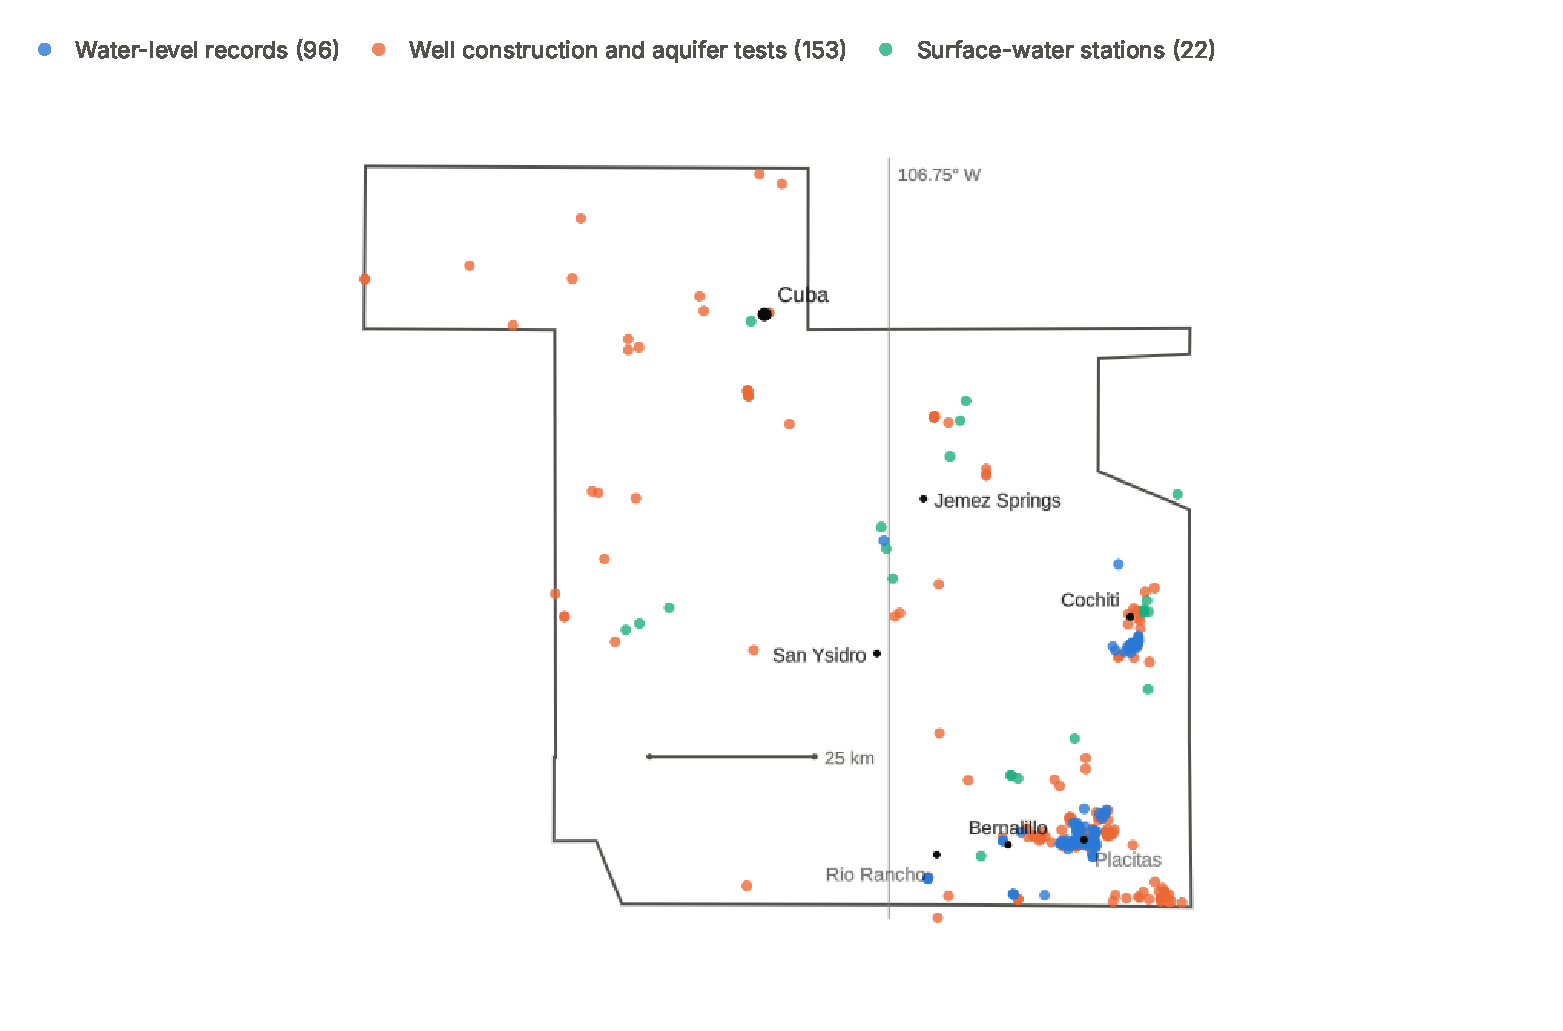
\includegraphics[width=0.82\textwidth]{county_coverage_map}
  \caption{Every mapped site in the project's datasets, colored by what it measures: water-level
  records (USGS monitoring wells and NMBGMR wells), well construction and aquifer tests (OSE aquifer
  tests and well logs), and surface-water stations (USGS stream, canal, and reservoir sites, including
  the Rio Puerco at Cuba). Most sites lie east of 106.75\textdegree{}\,W along the Rio Grande; within
  25\,km of Cuba there are only one-time aquifer tests, one well log, and one stream gage. A dot is a
  site with any record, not necessarily active monitoring. Outline: Sandoval County (simplified, US
  Census Bureau). Town locations approximate.}
  \label{fig:map}
\end{figure*}

% =====================================================================
\section{Study Area}\label{sec:study}
% =====================================================================
\subsection{Sandoval County}
\draftnote{Describe the county, its hydrogeologic settings, and its main communities and water
sources (Fig.~\ref{fig:map}).}

\subsection{Cuba Focus Area}
Cuba lies on the eastern edge of the San Juan Basin. The case study focuses on the Ojo Alamo
Sandstone and San Jose Formation near Cuba \citep{usgs_rasa_sjb,kernodle1996}. In this report,
the \emph{Cuba area} is the area within 25\,km of the village center; distances to Cuba are
straight-line distances from that center.
\draftnote{Describe Cuba, its water supply, and the aquifers it draws from.}

% =====================================================================
\section{Data}\label{sec:data}
% =====================================================================
Town-specific data for Cuba are limited, so the study relies on public datasets that can be
filtered to Sandoval County and the area around Cuba. Eight datasets were collected
(Table~\ref{tab:datasets}). For seven of them, a one-page brief records what the dataset contains,
which research questions it can help answer, which plots to make from it, and what it can't
show; a plotting guide compares all seven. The raw files are kept unedited in the project
repository \citep{team23_repo}.

% ---------------------------------------------------------------------
%  Table 1: datasets (full width; LaTeX places it at the top of a page)
% ---------------------------------------------------------------------
\begin{table*}[t]
  \caption{Datasets collected for the study. Distances are measured from Cuba.}
  \label{tab:datasets}
  \footnotesize
  \begin{tabularx}{\textwidth}{@{}>{\raggedright}p{0.9in}>{\raggedright}p{0.95in}
      >{\raggedright\arraybackslash}X>{\raggedright\arraybackslash}X l@{}}
    \toprule
    \textbf{Dataset} & \textbf{Source} & \textbf{Contents} & \textbf{Relevance to Cuba} & \textbf{Used for} \\
    \midrule
    Groundwater-level statistics & USGS & Monthly and yearly depth to water at 9 wells on 4 sites,
      1998--2026 & Wells are 65--95\,km away, in the eastern part of the county & RQ1, RQ5 \\
    Groundwater levels & NM Bureau of Geology & 456 depth-to-water measurements at 87 wells,
      1997--2019, with well depth & Nearest well is 38\,km away & RQ1, RQ2, RQ5 \\
    Aquifer tests & NM Office of the State Engineer & 179 tests in Sandoval County, 1930--2008:
      well construction, formation, and hydraulic properties & Includes tests at a well
      0.7\,km from Cuba & RQ2--RQ4 \\
    Wells with well logs & NM Office of the State Engineer & Drilling records for 6 Sandoval
      County wells, 1978--2022: borehole depth and depth to first water & Link to Cuba's wells
      not verified & RQ2, RQ5 \\
    Ojo Alamo Sandstone & USGS map atlas, 1990 & Maps of depth to the top of the sandstone, its
      thickness, and wells completed in it & Regional; covers the Cuba area & RQ4 \\
    San Jose Formation near Lindrith & NM Geological Society, 2025 & Water-bearing units,
      thickness of the Cuba Mesa Member, and groundwater levels & Centered near Lindrith, about
      30\,km north & RQ4 \\
    Rio Puerco at Cuba & USGS station 08332525 & 10 streamflow measurements (2019--2026) and
      4 gage-height readings & At Cuba, but measures the river, not groundwater & RQ3, RQ5 \\
    Aquifer sensitivity & NM Water Data & Sensitivity class for 613 mapped areas & Can't be
      located: the file has no coordinates & Not used \\
    \bottomrule
  \end{tabularx}
\end{table*}

\subsection{Datasets Used}
\subsubsection{Groundwater levels}
Two datasets measure depth to water below land surface, where a larger number means a lower
water table. The USGS statistics \citep{usgs_stats} give long monthly records for 9 wells at four
sites: Sandia, Lincoln Middle School in Rio Rancho, Bernalillo, and Dome Road. The same download also covers stream gages, canals, and
reservoirs, but only the groundwater records are used. The NM Bureau of Geology measurements
\citep{nmwd_levels} cover more wells but fewer years: most were measured in 1997--1998, and only
5 wells were measured again in 2016--2019, so few of them can show a long-term trend.

\subsubsection{Well and aquifer records}
The State Engineer's aquifer-test records \citep{ose_aquifertests} are the only dataset with
hydraulic properties, such as transmissivity and storativity, and they name the formation for
125 of the 179 tests. Seven test events name the Ojo Alamo Sandstone, among them 1957 and 1960
tests at what may be a single school well 0.7\,km from Cuba, but only one names the San Jose
Formation. The State Engineer's well logs \citep{ose_welllogs} add borehole depth and the depth at which
water was first found on the day each well was drilled, which is not a current water level.
\draftnote{Add the exact download page for the aquifer-test records.}

\subsubsection{Geology of the Cuba-area aquifers}
Two publications describe the formations studied for RQ4: a USGS map atlas of the Ojo Alamo
Sandstone across the San Juan Basin \citep{thorn1990}, and a study of the San Jose Formation near
Lindrith that identifies four water-bearing units and maps the Cuba Mesa Member
\citep{blandford2025}. Both are maps and reports rather than data tables, and neither shows which
formation Cuba's municipal wells draw from.

\subsubsection{Surface water at Cuba}
USGS station 08332525 on the Rio Puerco \citep{usgs_riopuerco} is the only dataset measured at
Cuba itself. Six of its 10 streamflow visits found no flow, and the other four measured 6.9 to
20.4 cubic feet per second. Because these are occasional visits rather than a continuous record,
the data are used only as context for the Cuba case study.

\subsubsection{Not used}
The aquifer sensitivity file \citep{nmwd_sensitivity} has no coordinates or shapes, so it can't be
mapped or matched to Cuba without its separate map layer, which was not obtained.

\subsection{Data Not Available}
The most important missing data are Cuba's municipal well records: well IDs, the formation each
well draws from, pumping volumes, and water-level history, held by the Village of Cuba or the
State Engineer \citep{nmose}. Every dataset brief identified these records as the missing piece for
RQ3. Also not obtained were the USGS digital aquifer data for the San Juan Basin
\citep{usgs_rasa_sjb}, groundwater-quality records such as the Brackish Water Assessment
\citep{nmbg_bwa}, acequia locations \citep{isc_acequias}, and records from other monitoring
networks \citep{ngwmn,cgmn}. Section~\ref{sec:limits} describes what their absence means for the
findings.

% =====================================================================
\section{Methods}\label{sec:methods}
% =====================================================================
\subsection{Data Cleaning}
Cleaning makes the data correct and consistent without drawing conclusions; averaging, trends,
and narrowing to the Cuba area happen in the analysis. Raw downloads are kept unedited. A MATLAB
script, \texttt{cleaning/clean\_csvs.m}, reads them and writes the cleaned files
(Table~\ref{tab:cleaned}), so anyone can rerun it and get the same result. As it runs, it prints
checks such as row counts, duplicate rows, and the list of formation names.

\begin{table}[t]
  \caption{Cleaned files produced so far.}
  \label{tab:cleaned}
  \footnotesize
  \begin{tabularx}{\linewidth}{@{}>{\raggedright}p{1.15in}r>{\raggedright\arraybackslash}X@{}}
    \toprule
    \textbf{File} & \textbf{Rows} & \textbf{Contents} \\
    \midrule
    \nolinkurl{groundwater_levels_monthly.csv} & 2,673 & Monthly mean depth to water at
      9 wells, June 1998 to September 2026 \\
    \nolinkurl{aquifer_tests.csv} & 179 & One row per aquifer test in Sandoval County, 1930 to
      2008, with 17 columns \\
    \bottomrule
  \end{tabularx}
\end{table}

\subsubsection{Shared conventions}
Every cleaned file starts with the same six columns: site ID, site name, latitude, longitude,
date, and source. Each has one row per measurement, sorted by site and date. Numbers are stored
without units or commas, dates are written as \mbox{YYYY-MM-DD}, and column names end with their unit,
such as \texttt{well\_depth\_ft}. Missing values are left blank rather than filled with
placeholders such as 0 or $-9999$, which a chart would plot as real values.

\subsubsection{Groundwater levels}
From the USGS statistics, the script keeps the depth-to-groundwater rows that are monthly means
and renames the columns to the shared names. Wells with an A or B suffix are kept as separate
sites, because they share a location but are measured at different depths. The cleaned file was
checked against the raw data: it has the same rows, dates, and values, with no duplicate
site-and-date rows.

\subsubsection{Aquifer tests}
The script keeps all 179 Sandoval County tests, including repeat tests on the same well, and the
16 raw columns the analysis needs: well construction, formation, water level, pumping rate, and
hydraulic properties. Empty and administrative columns are dropped. It converts numbers stored as
text, standardizes dates, and cleans formation names by trimming spaces, converting them to
uppercase, and fixing a misspelling. Three decisions were needed:
\begin{itemize}
  \item One hydraulic conductivity was recorded as a range, 11 to 21 ft/day; the midpoint,
        16 ft/day, is used.
  \item 104 tests list January 1, 1900, as the date of the starting water level, meaning the
        date is unknown, so that column is left out.
  \item 30 tests are dated January 1, which may mean only the year is known; they are kept as is.
\end{itemize}
Many tests are missing values, such as the formation (54 tests) and storativity (165 tests); these
cells are left blank.

\subsubsection{Open issues}
Most of the State Engineer's well IDs in the aquifer-test file are incomplete: 157 of the 179 are
partial, so the cleaned file has 73 site IDs for about 149 distinct wells. The analysis therefore
tells wells apart by name and location rather than by ID. The Bureau of Geology water levels, the
Rio Puerco measurements, and the well logs still need cleaning; the first and last of these also
need their UTM coordinates converted to latitude and longitude.
\draftnote{Update this paragraph once the remaining files are cleaned.}

\subsection{Analysis}
The analysis focuses on measurable indicators, such as depth to water, water-level change over
time, well depth, aquifer unit, and hydraulic properties from aquifer tests, rather than a full
hydrologic model. Where records
are sparse, the results say so instead of filling the gaps.
All analysis code is in the \texttt{analysis/} folder of the repository. Each chart is a Python
function that returns the figure together with its takeaway, caption, scope, and labeled findings,
so the app, this report, and the documentation show the same numbers; every chart is reproduced on
the documentation site's \href{https://pdjordj11.github.io/eng_220_aquifer_project/analysis/}{Analysis page}. Datasets not yet cleaned (NMBGMR water levels, the Rio
Puerco visits, and the OSE well logs) receive only minimal preparation in code, such as converting
UTM zone~13 coordinates to latitude and longitude; the raw files are never changed.

\emph{Water-level trends (RQ1).} Monthly mean depths to water were averaged into annual means,
using only years with at least 9 months of data. Each well's trend is Sen's slope (the median of all
pairwise slopes), and its significance is the Mann--Kendall test; a well is called falling or rising
only when $p<0.05$ \citep{helsel2020}. Trends are reported for the full record and for 2016--2025.
Because annual levels are serially correlated, the $p$-values and intervals are optimistic.

\emph{Wells and aquifer units (RQ2, RQ4).} Each well contributes one point: the median NMBGMR
reading, the first OSE aquifer test, or the depth where water was first found in a well log. Wells
were grouped by the nearest of seven towns. Aquifer-test properties were compared by recorded
formation, using one median per well. The scanned USGS map of the Ojo Alamo Sandstone
\citep{thorn1990} was read by eye, not digitized.

\emph{Cuba case study (RQ3).} The ``Cuba area'' is defined as within 25\,km of the village center.
For every dataset, we measured the distance from Cuba to its nearest site and recorded what kind of
record it holds.

\emph{Coverage and indicators (RQ5, RQ6).} Every site in every dataset was mapped and counted by
year to show where and when monitoring exists, and each dataset was rated against each research
question from its brief. Indicators were kept only where they can be computed from the data, each
with the place it applies to and a stated confidence.

\subsection{Classifying Findings}
Each finding is labeled as one of the following:
\begin{itemize}
  \item \textbf{Measured:} a trend or pattern the data show directly.
  \item \textbf{Hypothesis:} a possible explanation the data are consistent with but don't prove.
  \item \textbf{Insufficient data:} a question the available records can't answer yet.
\end{itemize}

\subsection{Interactive Dashboard}
Results are presented in an interactive Streamlit dashboard built with pandas and Plotly. Code
and documentation are maintained on GitHub \citep{team23_repo}. The dashboard uses the same chart
functions as this report. Besides a home page, it has five pages: a county map of every site; the
groundwater-level records and trends (RQ1); well depth, depth to water, and aquifer properties by
area and formation (RQ2, RQ4); the Cuba case study (RQ3, RQ4); and data sources with monitoring
coverage and the groundwater-stress indicators (RQ5, RQ6). Each chart is shown with its takeaway,
its scope (Cuba, the Cuba area, or Sandoval County), a caption, its labeled findings, and the data
behind it, which visitors can download. Charts can be zoomed and hovered for exact values.
\draftnote{Dashboard lead: update this paragraph if the app's pages change before Nov 10.}

% =====================================================================
\section{Results}\label{sec:results}
% =====================================================================
\subsection{Groundwater Levels}
\begin{figure*}[t]
  \centering
  % Made by analysis/charts.py (groundwater_hydrographs); remake with `python -m analysis.export_figures`.
  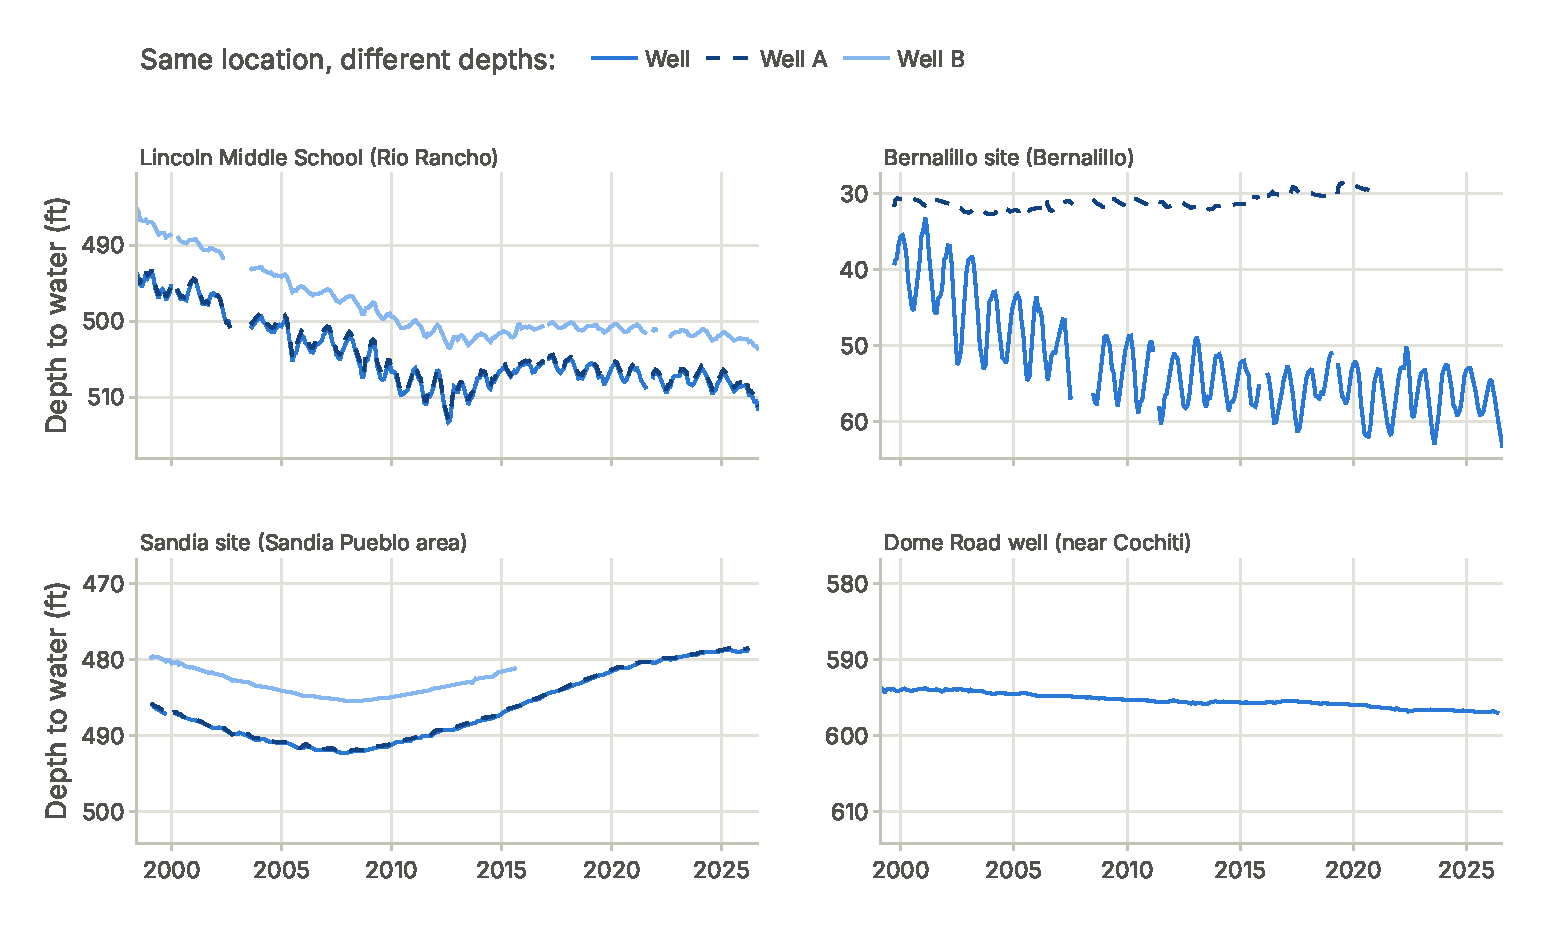
\includegraphics[width=\textwidth]{groundwater_hydrographs}
  \caption{Monthly mean depth to water at the nine USGS monitoring wells, 1998--2026 (axis flipped:
  up is a higher water table). Wells marked A or B share a location but are measured at a different
  depth. Every panel spans the same vertical range, so steepness can be compared. Five of the nine
  wells fell over their records; at the Sandia site the water level has risen about 13\,ft since 2007.
  Scope: Sandoval County, 65--95\,km from Cuba (not Cuba). Source: USGS Water Data statistics,
  parameter 72019, cleaned by J.~Wauneka.}
  \label{fig:levels}
\end{figure*}
The nine USGS monitoring wells sit at four sites between Rio Rancho and Cochiti, 65--95\,km from
Cuba (Fig.~\ref{fig:levels}). Over their full records, five wells fell, three rose, and one showed
no clear trend. Water levels at Lincoln Middle School (Rio Rancho) fell 0.36--0.40\,ft per year and
were still falling in 2016--2025, as was the Dome Road well near Cochiti. The Bernalillo site's main
well fell about 0.5\,ft per year over its record but showed no clear trend in 2016--2025. At the
Sandia site the water level fell until 2007 and then rose about 13\,ft by 2025 (\emph{Measured}).
That recovery coincides with the San Juan--Chama Drinking Water Project, after which the Albuquerque
water utility pumped less groundwater and water levels rose across the Albuquerque area
\citep{ritchie2019}; these data alone cannot show the cause (\emph{Hypothesis}).

In the Placitas area, only five NMBGMR wells were measured both in 1997--98 and in 2018--19. Three
changed by 5\,ft or less (two of them from baselines flagged as recently pumped), one (PC-014) is 51\,ft deeper, and one (PC-025) is 57\,ft shallower;
PC-025's 1990s readings rose steadily after a first reading flagged as recently pumped, so its
1990s average is not a stable baseline. Five wells cannot establish an area-wide trend
(\emph{Insufficient data}).

\subsection{Wells and Aquifer Units}
\begin{figure*}[t]
  \centering
  % Made by analysis/charts.py (well_depth_vs_water); remake with `python -m analysis.export_figures`.
  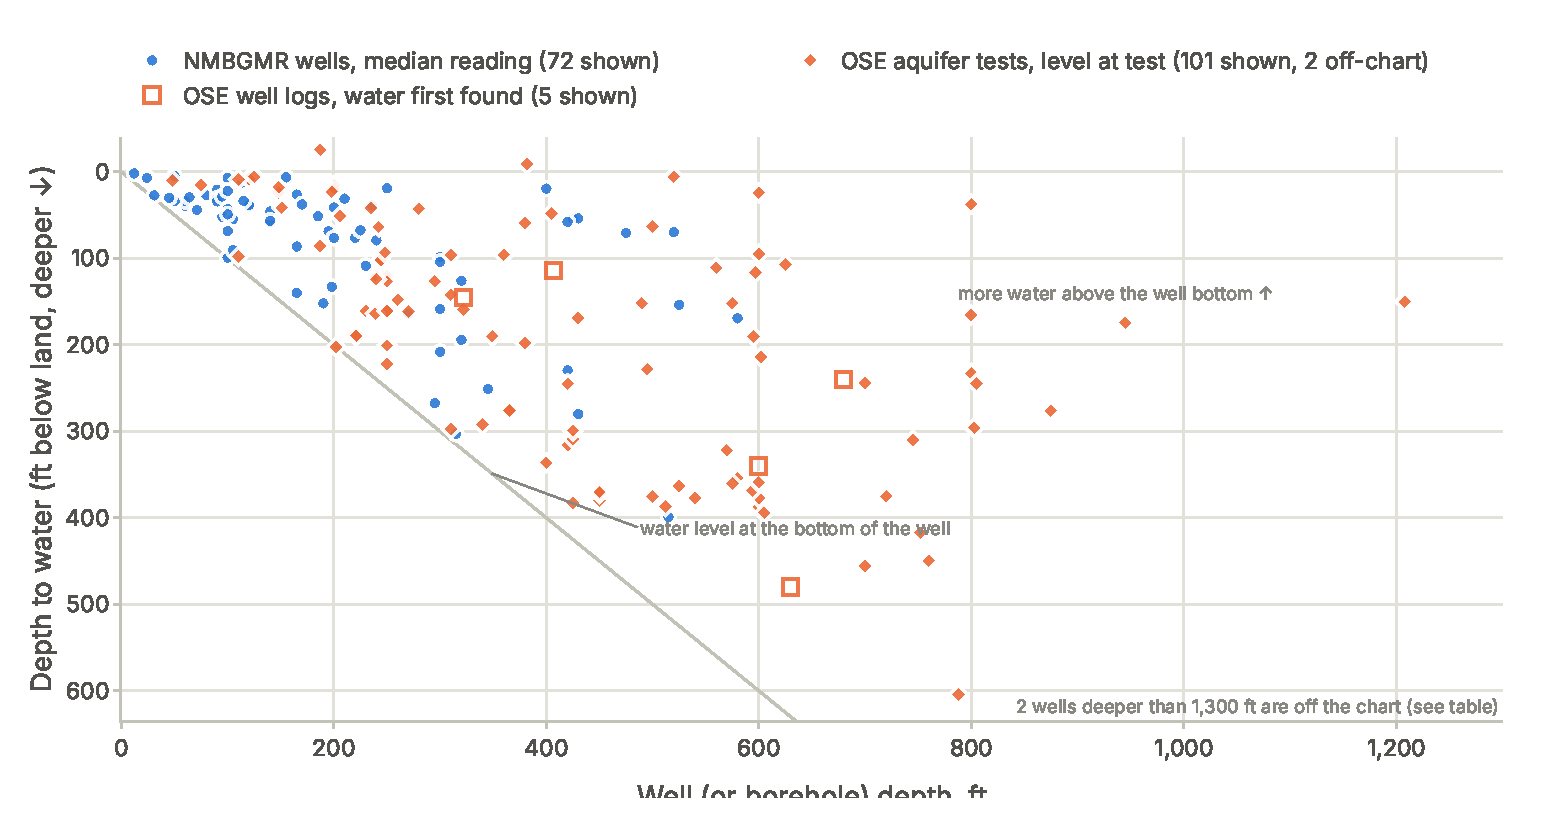
\includegraphics[width=0.72\textwidth]{well_depth_vs_water}
  \caption{Well depth against depth to water, one point per well, from three record types,
  1930--2022. The record types measure water differently (a 1997--2019 reading, the level on the
  day of an aquifer test, and the depth where water was first found during drilling), so they are
  context rather than one comparable series. Scope: Sandoval County, including 7 wells within
  25\,km of Cuba. Sources: NMBGMR groundwater levels; NM OSE aquifer tests and well logs.}
  \label{fig:depth}
\end{figure*}
Where water is deeper, wells are drilled deeper (Spearman $\rho=0.63$--$0.64$ within the two larger
record types; Fig.~\ref{fig:depth}), but the spread is wide: half of 180 wells have water between 41 and 241\,ft below land.
Among recorded wells, depth to water was smallest around Cochiti--Pe\~{n}a Blanca and largest around
Bernalillo--Rio Rancho, though the groups mix record types and decades. Aquifer properties vary
widely: within three formations, transmissivity values span more than the spread between formation
medians, up to almost five orders of magnitude in the Madera Limestone. Only the aquifer-test file records the formation, so the other well
records cannot be assigned to an aquifer unit (\emph{Insufficient data}).

\subsection{Cuba Case Study}
\begin{figure*}[t]
  \centering
  % Made by analysis/charts.py (cuba_nearest_records); remake with `python -m analysis.export_figures`.
  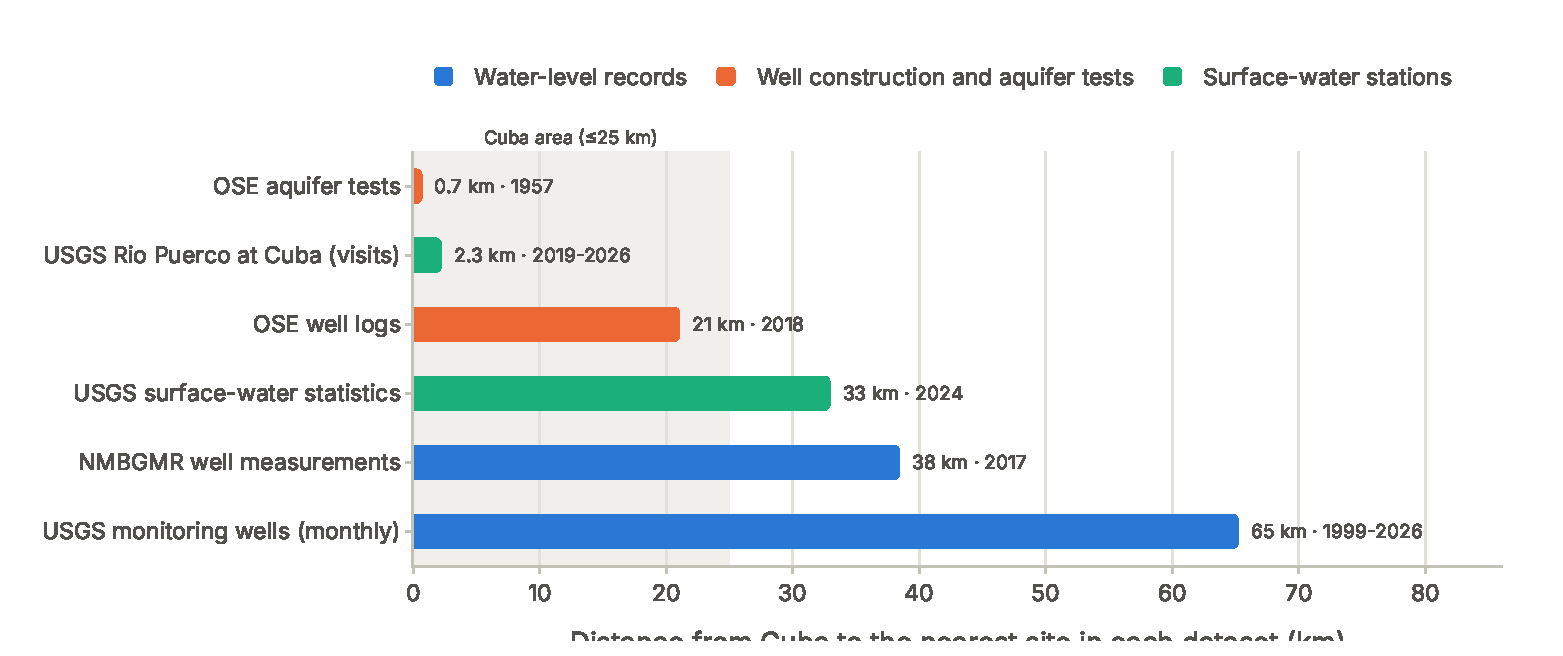
\includegraphics[width=0.8\textwidth]{cuba_nearest_records}
  \caption{Distance from Cuba to the nearest site in each dataset. The nearest well with repeated
  water-level measurements is 38\,km away; within 25\,km there are only one-time aquifer tests
  (1957--1979), one well log, and the Rio Puerco stream gage. Distances are straight-line from the
  approximate village center. Sources: USGS monitoring wells and surface-water statistics, NMBGMR
  groundwater levels, NM OSE aquifer tests and well logs, and USGS station 08332525.}
  \label{fig:nearest}
\end{figure*}
Within 25\,km of Cuba, the collected data contain 15 wells with one-time aquifer tests
(1957--1979), one well log (2018), and the Rio Puerco stream gage. Nine of the tested wells recorded
a depth to water on test day, but no well near Cuba has been measured repeatedly; the nearest well
with repeated water-level measurements is 38\,km away, and the nearest USGS monitoring well 65\,km
(Fig.~\ref{fig:nearest}). The data therefore cannot confirm or rule out severe decline in Cuba's
aquifer (\emph{Insufficient data}). Answering RQ3 requires Cuba's municipal well records: well IDs,
producing formations, pumping volumes, and water-level histories.

\begin{figure*}[t]
  \centering
  % Made by analysis/charts.py (ojo_alamo_vs_san_jose); remake with `python -m analysis.export_figures`.
  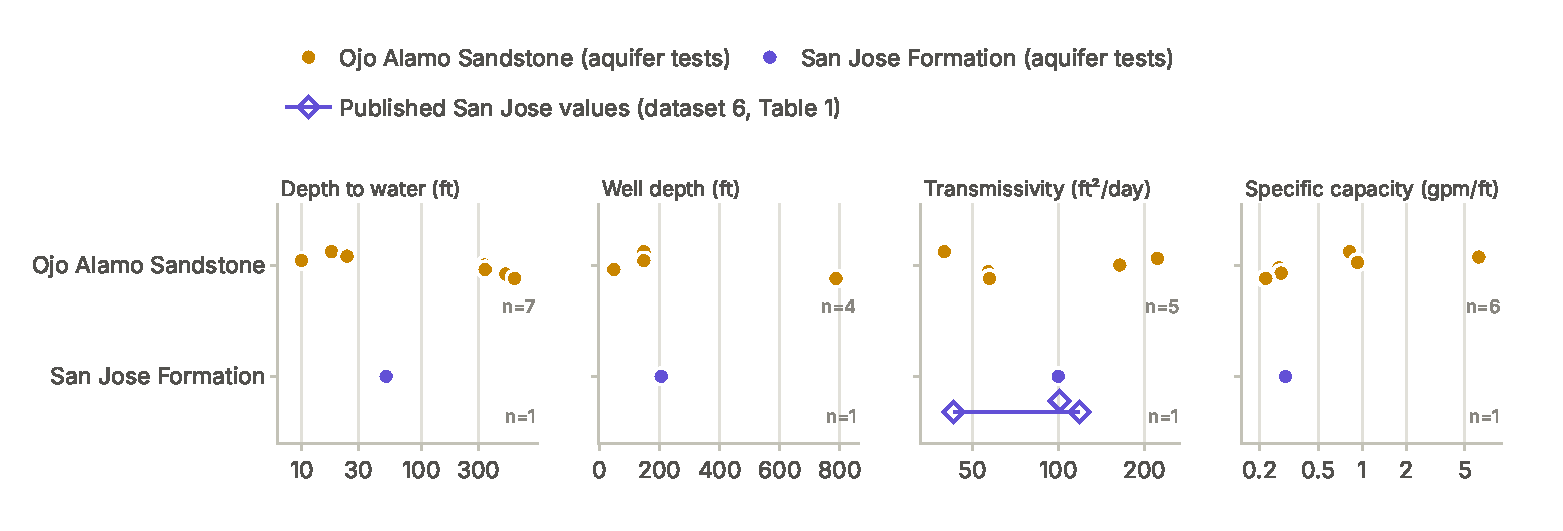
\includegraphics[width=\textwidth]{ojo_alamo_vs_san_jose}
  \caption{Every aquifer test that names the Ojo Alamo Sandstone (seven events) or the San Jose
  Formation (one), 1953--1977, with published San Jose transmissivity values compiled by
  \citet{blandford2025} (open diamonds). Depth to water, transmissivity, and specific capacity use
  log scales. Scope: tests 1--45\,km from Cuba. Source: NM OSE aquifer tests.}
  \label{fig:formations}
\end{figure*}
On the USGS map of the Ojo Alamo Sandstone \citep{thorn1990}, Cuba sits at the southeastern end of
the formation's outcrop, where it is shallow, and its top deepens northward past 1{,}000 and
3{,}000\,ft. Only eight aquifer-test events in the county name the Ojo Alamo (seven) or the San Jose
Formation (one), all from 1953--1977: too few to describe either formation, let alone compare them
(Fig.~\ref{fig:formations}).
The single San Jose test (100\,ft$^2$/day) is close to the one published Cuba Mesa Member value near
Lindrith and within a San Jose range from earlier tests, both compiled by \citet{blandford2025}.

As surface-water context, not evidence about groundwater, the Rio Puerco at Cuba had measurable
flow on all four visits in April and May and on none of the six visits from August to March,
2019--2026 \citep{usgs_riopuerco}. Spot visits cannot show how often the river runs dry.

\subsection{Monitoring Coverage and Data Gaps}
\begin{figure*}[t]
  \centering
  % Made by analysis/charts.py (coverage_timeline); remake with `python -m analysis.export_figures`.
  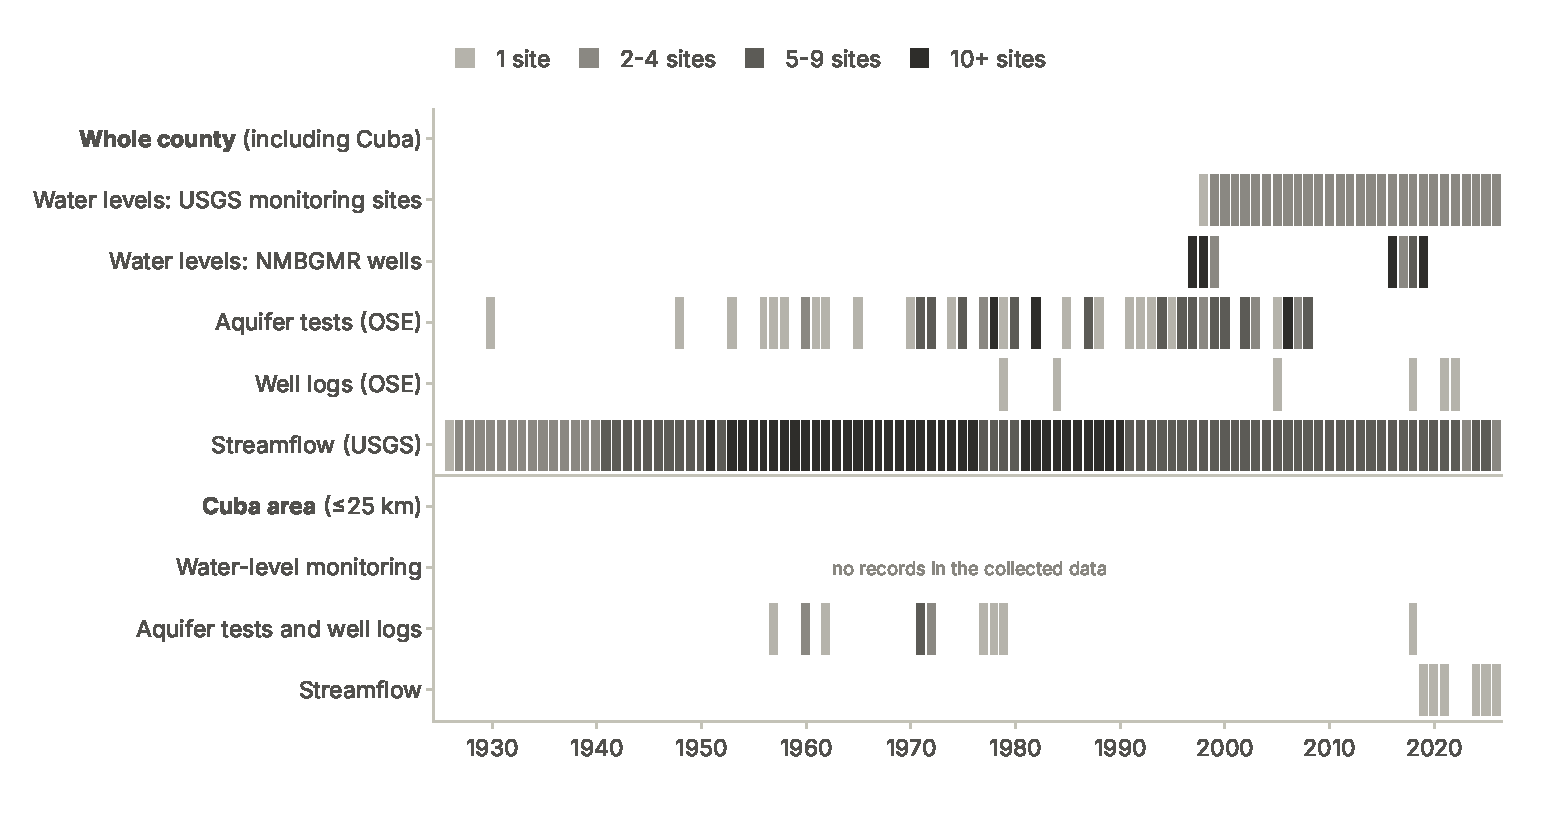
\includegraphics[width=0.85\textwidth]{coverage_timeline}
  \caption{Number of sites with at least one record in each year, 1926--2026, for the whole county
  (top) and the Cuba area within 25\,km (bottom). Darker shading means more sites. Gaps are years
  with no record in the collected files; other agencies may hold data. Sources: USGS, NMBGMR, and
  NM OSE.}
  \label{fig:coverage}
\end{figure*}
Monitoring is concentrated along the Rio Grande: 86\% of the 271 mapped sites lie east of
106.75\textdegree{}\,W (Fig.~\ref{fig:map}). Groundwater levels have been monitored every year only
since 1999, and only at four sites in the east of the county; the collected data have no
water-level monitoring in the Cuba area (Fig.~\ref{fig:coverage}). According to the dataset briefs, no dataset gives more than
limited support for RQ3, the question about Cuba itself.

\subsection{Groundwater-Stress Indicators}
Five indicators can be computed from the collected data without overstating their certainty: the
2016--2025 water-level trend at the monitored wells (four of the seven wells with enough recent data
were falling and two rising), the full-record water-level change at the same wells ($-16$ to
$+8$\,ft), the distance from Cuba to the nearest repeated water-level record (38\,km), the share of
Rio Puerco visits with flow (4 of 10, river only), and the number and age of aquifer tests near Cuba
(15 wells, 1957--1979). Each applies only where its data were collected, and none measures how much
groundwater is left; the Streamlit app lists them with their scope and confidence (RQ6).

% =====================================================================
\section{Discussion}\label{sec:discussion}
% =====================================================================
\draftnote{What the results mean for Sandoval County and Cuba, and which indicators best
communicate groundwater stress (RQ6).}

% =====================================================================
\section{Limitations}\label{sec:limits}
% =====================================================================
The project proposal included three questions that this report does not answer, because the data
needed for them were not obtained during the project:
\begin{itemize}
  \item \textbf{Groundwater quality and salinity.} No groundwater-quality records were collected.
        The water-quality measurements in the USGS file all come from streams, mainly the Rio
        Grande below Cochiti Dam, far from Cuba.
  \item \textbf{Acequias.} No data on acequia locations or service areas were collected.
  \item \textbf{Groundwater and surface-water links.} Comparing the two requires repeated
        water-level measurements near a stream. The only stream records at Cuba are 10 visits to
        the Rio Puerco gage, and the nearest well in the water-level datasets is 38\,km
        away.
\end{itemize}
The data that were collected also limit what the results can support:
\begin{itemize}
  \item Almost nothing measures Cuba's groundwater: the nearest well measured more than once is
        38\,km away, so RQ3 cannot be answered with these data.
  \item Four monitoring sites carry the county's trend results; they are indicators at those
        points, not a county average or a measure of remaining supply.
  \item Most aquifer tests are decades old and record conditions on the day of the test, and only
        eight name the Ojo Alamo Sandstone or San Jose Formation.
  \item No geologic-region layer was available, so wells are grouped by nearest town and by the
        formation named in aquifer tests.
  \item Trend tests assume independent years; serial correlation makes them look more certain than
        they are.
\end{itemize}

% =====================================================================
\section{Conclusions}\label{sec:conclusions}
% =====================================================================
\draftnote{Summary of findings and recommended next steps.}

% =====================================================================
%  Back matter
% =====================================================================
\Needspace{9\baselineskip}
\section*{Data and Code Availability}
\begin{description}[style=nextline,leftmargin=1em,itemsep=1pt,font=\normalfont\bfseries]
  \item[Code and data] \href{https://github.com/pdjordj11/eng_220_aquifer_project}{\nolinkurl{github.com/pdjordj11/eng_220_aquifer_project}}
  \item[Interactive dashboard] \href{https://eng220aquiferproject.streamlit.app/}{\nolinkurl{eng220aquiferproject.streamlit.app}}
  \item[Documentation] \href{https://pdjordj11.github.io/eng_220_aquifer_project/}{\nolinkurl{pdjordj11.github.io/eng_220_aquifer_project}}
\end{description}

\section*{Author Contributions}
\begin{description}[leftmargin=0pt,labelsep=0.4em,itemsep=0pt,font=\normalfont\bfseries]
  \item[P.~Djordjevic:] documentation, final report, presentation, and video.
  \item[D.~Gonzales:] data acquisition: collected seven datasets and wrote a research brief for
        each, plus a plotting guide comparing them.
  \item[J.~Wauneka:] data cleaning: wrote the MATLAB script that produces the cleaned
        groundwater-level and aquifer-test files.
  \item[M.~Watkins:] analysis code and visualizations: wrote the analysis package (data loaders,
        trend statistics, and 15 charts with labeled findings) that feeds the app, this report's
        figures, and the documentation site.
  \item[M.~Yousef:] GitHub workflow and the Streamlit app.
\end{description}

\section*{Acknowledgments}
\draftnote{To be written.}

\bibliographystyle{plainnat}
\bibliography{references}

\end{document}
